\documentclass[runningheads]{llncs}

\setlength{\paperheight}{232.8mm}
\setlength{\paperwidth}{151.5mm}
\setlength\voffset     {-23mm}
\setlength\hoffset     {-34mm}

%
\usepackage{hyperref}
\usepackage{multicol}
\usepackage[final]{changes}
\usepackage{url}
\usepackage{amsmath}
\usepackage{bm}
\usepackage{multirow}
\usepackage{tcolorbox}
\usepackage{rotating}
\usepackage{latexsym,amssymb,amsmath}
\usepackage{makecell}
\usepackage{xspace}
\usepackage{paralist}
\usepackage{wrapfig}
\usepackage{adjustbox}
\usepackage{cite}
%\usepackage{times}
%%%%%%%%%%%%%%%%%%%%%%%%%%%%%%%%%%%%%%%%%%%%%%%%%%%%%%%%%%%%%%%%%%%%%%%%%%%%%%
%%% Time-stamp: "2018-09-07 18:35:03 calvanese"
%%%%%%%%%%%%%%%%%%%%%%%%%%%%%%%%%%%%%%%%%%%%%%%%%%%%%%%%%%%%%%%%%%%%%%%%%%%%%%

%%%%%%%%%%%%%%%%%%%%%%%%%% General Math

\newcommand{\A}{\ensuremath{\mathcal{A}}}
\newcommand{\B}{\ensuremath{\mathcal{B}}}
%\newcommand{\C}{\ensuremath{\mathcal{C}}}
\newcommand{\D}{\ensuremath{\mathcal{D}}}
\newcommand{\E}{\ensuremath{\mathcal{E}}}
\newcommand{\F}{\ensuremath{\mathcal{F}}}
%\newcommand{\G}{\ensuremath{\mathcal{G}}}
\renewcommand{\H}{\ensuremath{\mathcal{H}}}
\newcommand{\I}{\ensuremath{\mathcal{I}}}
\newcommand{\J}{\ensuremath{\mathcal{J}}}
\newcommand{\K}{\ensuremath{\mathcal{K}}}
\renewcommand{\L}{\ensuremath{\mathcal{L}}}
\newcommand{\M}{\ensuremath{\mathcal{M}}}
\newcommand{\N}{\ensuremath{\mathcal{N}}}
\renewcommand{\O}{\ensuremath{\mathcal{O}}}
\renewcommand{\P}{\ensuremath{\mathcal{P}}}
\newcommand{\Q}{\ensuremath{\mathcal{Q}}}
\newcommand{\R}{\ensuremath{\mathcal{R}}}
%\renewcommand{\S}{\ensuremath{\mathcal{S}}}
\newcommand{\T}{\ensuremath{\mathcal{T}}}
%\newcommand{\U}{\ensuremath{\mathcal{U}}}
\newcommand{\V}{\ensuremath{\mathcal{V}}}
\newcommand{\W}{\ensuremath{\mathcal{W}}}
\newcommand{\X}{\ensuremath{\mathcal{X}}}
\newcommand{\Y}{\ensuremath{\mathcal{Y}}}
\newcommand{\Z}{\ensuremath{\mathcal{Z}}}

%%%%%%%%%%%%%%%%%%%%%%%%%% Abbreviations

%%\newcommand{\eset}{\emptyset}
%%\newcommand{\col}{\colon}
\newcommand{\ol}[1]{\overline{#1}}                % overline
%\newcommand{\ul}[1]{\underline{#1}}               % underline
%%\newcommand{\uls}[1]{\underline{\raisebox{0pt}[0pt][0.45ex]{}#1}}
%% ul with space between text and line

\newcommand{\ra}{\rightarrow}
\newcommand{\Ra}{\Rightarrow}
\newcommand{\la}{\leftarrow}
\newcommand{\La}{\Leftarrow}
%\newcommand{\lra}{\leftrightarrow}
\newcommand{\Lra}{\Leftrightarrow}
\newcommand{\lora}{\longrightarrow}
\newcommand{\Lora}{\Longrightarrow}
\newcommand{\lola}{\longleftarrow}
\newcommand{\Lola}{\Longleftarrow}
\newcommand{\lolra}{\longleftrightarrow}
\newcommand{\Lolra}{\Longleftrightarrow}
%\newcommand{\ua}{\uparrow}
\newcommand{\Ua}{\Uparrow}
\newcommand{\da}{\downarrow}
\newcommand{\Da}{\Downarrow}
\newcommand{\uda}{\updownarrow}
\newcommand{\Uda}{\Updownarrow}

%%%%%%%%%%%%%%%%%%%%%%%%%% Relations

%%\newcommand{\incl}{\subseteq}
%%\newcommand{\imp}{\rightarrow}
\newcommand{\per}{\mbox{\bf .}}                  % period

%%%%%%%%%%%%%%%%%%%%%%%%%% Delimiters

%%\newcommand{\quotes}[1]{{\lq\lq #1\rq\rq}}
%\newcommand{\set}[1]{\{#1\}}                      % set
%\newcommand{\Set}[1]{\left\{#1\right\}}
\newcommand{\bigset}[1]{\Bigl\{#1\Bigr\}}
\newcommand{\bigmid}{\Big|}
\newcommand{\size}[1]{|{#1}|}                     % cardinality of a set
%%\newcommand{\Card}[1]{\left| #1\right|}
\newcommand{\card}[1]{\sharp #1}
\newcommand{\tup}[1]{\langle #1\rangle}            % tuple
\newcommand{\Tup}[1]{\Braket{#1}}
\newcommand{\norm}[2]{\|#1\|_{#2}}
\newcommand{\setone}[2][1]{\set{#1\cld #2}}

%%%%%%%%%%%%%%%%%%%%%%%%%% STYLING AND SPACING

%\newcommand{\inlinetitle}[1]{\smallskip\noindent\textbf{#1.}\xspace}





\newcolumntype{C}{>{\centering\arraybackslash}X}

%\makeatletter
%\g@addto@macro\normalsize{%
%\setlength{\abovecaptionskip}{-2pt}
%\setlength{\belowcaptionskip}{12pt}
%\setlength\abovedisplayskip{3pt}
%\setlength\belowdisplayskip{3pt}
%\setlength\abovedisplayshortskip{3pt}
%\setlength\belowdisplayshortskip{3pt}
%}
%\makeatother

\newcounter{dummy} 
\newcounter{dummy1} 
\newcounter{dummy2}
\newcounter{dummy3} 
\newcounter{dummy4}
\newcounter{dummy5} 
\newcounter{dummy6}
\newcounter{dummy7}
%\numberwithin{dummy}{section}

\usepackage[thmmarks,amsmath]{ntheorem}
%\theorempreskip{1pt}
%\theorempostskip{1pt}

%\theoremstyle{plain}
%\theorembodyfont{\normalfont}
%\theoremseparator{.}
%\let\definition\relax
%\theoremsymbol{\ensuremath{\square}}
%\newtheorem{definition}{Definition}


\let\proposition\relax
\let\theorem\relax
\let\lemma\relax
\let\definition\relax
\theoremseparator{.}
\theorembodyfont{\itshape}
\theoremsymbol{$\triangleleft$}
\newtheorem{theorem}[dummy]{Theorem}
\newtheorem{definition}[dummy2]{Definition}
\newtheorem{proposition}[dummy3]{Proposition}

\usepackage{booktabs}
\usepackage{apptools}
\usepackage{chngcntr}
\newtheorem{lemma}[dummy1]{Lemma}

\let\remark\relax
\let\example\relax
%\let\example*\relax
\theorembodyfont{\normalfont}
\newtheorem{example}[dummy4]{Example}
\newtheorem{remark}[dummy5]{Remark}
%\newtheorem{example*}[dummy4]{Example}


\theoremstyle{nonumberplain}
\theoremheaderfont{\itshape}
\theorembodyfont{\normalfont}
\let\proof\relax
\theoremseparator{.}
\theoremsymbol{\ensuremath{\dashv}}
\newtheorem{proof}[dummy6]{Proof}


\qedsymbol{\ensuremath{\dashv}}


%%% Local Variables:
%%% mode: latex
%%% TeX-master: "main"
%%% save-place: t
%%% End:

\usepackage{todonotes}

\usepackage{graphicx}
\usepackage{xcolor,color}
\usepackage{subfig}
\usepackage{tikz}
\usepackage{calc}

\usepackage{tabularx}
\usepackage{booktabs}

\usepackage{ulem}

\usepackage{kbordermatrix}
\usepackage{amsmath,amsfonts}
\usepackage{braket}
\usepackage{xfrac}

\usepackage{pifont}
\usepackage{amssymb}
\usepackage{paralist}
\usepackage[inline]{enumitem}

\newcommand{\pmin}{\rho}

\newcommand{\const}[1]{\mathsf{#1}}

\newcommand{\alphabet}{\Sigma}
\newcommand{\tasks}{\mathcal{A}}
\newcommand{\hidden}{\tau}

\newcommand{\uswn}{SWN\xspace}
\newcommand{\net}{\ensuremath{N}}
\newcommand{\tg}{\ensuremath{G}}
\newcommand{\closed}[1]{\overline{#1}}
\newcommand{\marking}{m}
\newcommand{\enaset}[2]{E_{#2}(#1)}
\newcommand{\fire}[4]{#1\xrightarrow{#2}_{#4}#3}
\newcommand{\probt}[3]{\mathbb{P}_{#2,#3}(#1)}
\newcommand{\prob}[2]{\mathbb{P}_{#2}(#1)}
\newcommand{\rg}[1]{RG(#1)}
\newcommand{\ind}[1]{\textnormal{\texttt{#1}}}
\newcommand{\seq}{\eta}
\newcommand{\run}{\xi}
\newcommand{\trace}{\sigma}
\newcommand{\traces}[1]{\mathit{traces}(#1)}
\newcommand{\ptraces}[2]{\mathit{ptraces}_{#2}(#1)}

\newcommand{\nreach}[3][]{#2 \overset{#1}{\rightsquigarrow} #3}
\newcommand{\runs}[2]{runs_{#2}(#1)}
\newcommand{\seqs}[2]{seqs_{#2}(#1)}
\newcommand{\transp}[1]{#1^\top}
\newcommand{\embed}{\phi}
\newcommand{\trembed}{{\embed^{\text{tr}}}}
\newcommand{\gorgembed}{{\embed^{g}}}


\newcommand{\pa}{\rho_{23}}
\newcommand{\pb}{\rho_{24}}
\newcommand{\pc}{\rho_{55}}
\newcommand{\pd}{\rho_{65}}
\newcommand{\pe}{\rho_{67}}
\newcommand{\pf}{\rho_{57}}

\newcommand{\logtrace}{\trace}
\newcommand{\nonlogtrace}{{\trace^\star}}
\newcommand{\DeclModel}{\mathcal{D}}
\newcommand{\Activities}{A}
\newcommand{\DeclConstr}{\Pi}
\newcommand{\TraceOf}[1]{\textit{Trace}(#1)}
\newcommand{\InvInterp}[1]{\mathcal{I}^{-1}(#1)}

\newcommand{\approptoinn}[2]{\mathrel{\vcenter{
			\offinterlineskip\halign{\hfil$##$\cr
				#1\propto\cr\noalign{\kern2pt}#1\sim\cr\noalign{\kern-2pt}}}}}
\newcommand{\appropto}{\mathpalette\approptoinn\relax}


\newcommand{\unravelled}{unfolded}
\newcommand{\unravelling}{unfolding}
\newcommand{\unravel}{unfold}



%
%\def\WWITHN{def}
%\ifdefined\WWITHN
%\newcommand{\WCal}[2]{{\mathcal{W}_{#1}^{#2}}}
%\newcommand{\TBf}[2]{{\mathbf{T}_{#1}^{#2}}}
%\else
\newcommand{\TBf}[2]{{\mathbf{G}_{#1}}}
%\fi
\newcommand{\expN}{\closed{\tg_{\rg{\net}}}}

\def\EqualityHolds{itholds}
\ifdefined\EqualityHolds
\newcommand{\probarg}{\net}
\newcommand{\WCal}[2]{\ptraces{\net}{#1}}
\else
\newcommand{\probarg}{\expN}
\newcommand{\WCal}[2]{\ptraces{\closed{\tg_{\rg{\net}}}}{#1}}
\fi
\newcommand{\probskip}[1]{\prob{#1}{\probarg}}
\newcommand{\goldenrank}{\mathcal{R}} 
\usepackage{stmaryrd}
\newcommand{\sem}[1]{\ensuremath{\llbracket #1 \rrbracket}}

\newcommand{\LTL}{\ensuremath{\text{LTL}}\xspace}
\newcommand{\LTLf}{\ensuremath{\text{LTL}_f}\xspace}
\newcommand{\PLTL}{\ensuremath{\text{PLTL}_f}\xspace}
\newcommand{\PLTLz}{\ensuremath{\text{PLTL}_f^0}\xspace}

\newcommand{\Wuntil}{\mathcal{W}}

\newcommand{\At}{\ensuremath{\mathsf{At}}\xspace}

\newcommand{\nats}{\ensuremath{\mathbb{N}}\xspace}
\newcommand{\acc}{\ensuremath{\mathsf{acc}}\xspace}
\newcommand{\branch}{\ensuremath{\mathsf{b}}\xspace}
\newcommand{\exa}{\ensuremath{\mathsf{exa}}\xspace}
\newcommand{\ini}{\ensuremath{\mathsf{in}}\xspace}
\newcommand{\ms}{\ensuremath{\mathsf{m}}\xspace}
\newcommand{\wt}{\ensuremath{\mathsf{wt}}\xspace}
%\newcommand{\run}{\ensuremath{\mathsf{run}}\xspace}
\newcommand{\rnk}{\ensuremath{\mathsf{rk}}\xspace}
\newcommand{\swt}{\ensuremath{\mathsf{w}}\xspace}
\newcommand{\csub}{\ensuremath{\mathsf{csub}}\xspace}
\newcommand{\END}{\ensuremath{\mathsf{END}}\xspace}

\newcommand{\atom}{\ensuremath{\mathbf{a}}\xspace}

\newcommand{\Amc}{\ensuremath{\mathcal{A}}\xspace}
\newcommand{\Bmc}{\ensuremath{\mathcal{B}}\xspace}
\newcommand{\Imc}{\ensuremath{\mathcal{I}}\xspace}
\newcommand{\Lmc}{\ensuremath{\mathcal{L}}\xspace}
\newcommand{\Omc}{\ensuremath{\mathcal{O}}\xspace}
\newcommand{\Pmc}{\ensuremath{\mathcal{P}}\xspace}
\newcommand{\Qmc}{\ensuremath{\mathcal{Q}}\xspace}
\newcommand{\Smc}{\ensuremath{\mathcal{S}}\xspace}
\newcommand{\Wmc}{\ensuremath{\mathcal{W}}\xspace}

\newcommand{\Imf}{\ensuremath{\mathfrak{I}}\xspace}

\newcommand{\PS}{\text{\sc{PSpace}}\xspace}
\newcommand{\ET}{\text{\sc{ExpTime}}\xspace}

%\newcommand{\prob}[1]{\ensuremath{\scaleobj{1.2}{\circledcirc}_{#1}}\xspace}

\newcommand{\argmax}{\text{argmax}\xspace}
\newcommand{\declare}{Declare\xspace}
\newcommand{\pdeclare}{ProbDeclare\xspace}
\newcommand{\constraint}[1]{\texttt{#1}}
\newcommand{\activity}[1]{\ensuremath{\mathsf{#1}}}
%\newtheorem{theorem}{Theorem}
%\newtheorem{lemma}[theorem]{Lemma}
%\newtheorem{claim}[theorem]{Claim}
%\newtheorem{proposition}[theorem]{Proposition}
%\newtheorem{corollary}[theorem]{Corollary}
%\theoremstyle{definition}
%\newtheorem{example}[theorem]{Example}
%\newtheorem{definition}[theorem]{Definition}



%% temporal operators
\newcommand{\Next}{{\ensuremath\raisebox{0.25ex}{\text{\scriptsize$\bigcirc$}}}}
\newcommand{\Until}{\ensuremath{\mathbin{\mathcal{U}}}}
\newcommand{\Release}{\ensuremath{\mathbin{\mathcal{R}}}}
\newcommand{\Wntil}{\ensuremath{\mathbin{\mathcal{W}}}}









\allowdisplaybreaks

%%%%%%%%%%%%%%%%%%%%%%%%%%%%%
%%%%%%%  Conference / arXiv Versions  %%%%%%%
\newif\iffull\fulltrue
%\fullfalse		%%% uncomment to make conference version
\newcommand{\FullT}[1]{\iffull #1 \fi}
\newcommand{\FullF}[1]{\iffull \else #1 \fi}
\newcommand{\FullTF}[2]{\iffull #1 \else #2 \fi}
\usepackage{tkz-graph}
\usetikzlibrary{matrix,automata,arrows,calc,fit}
\usetikzlibrary{decorations.pathreplacing,positioning}


\definecolor{deepblue}{HTML}{0C3B80}
\definecolor{deepgreen}{HTML}{2EA601}
%\definecolor{deepblue}{HTML}{232F3E}
%\definecolor{chaptercolor}{HTML}{232F3E}{0.8}
\definecolor{lightOrange}{HTML}{FFA03C}
\definecolor{darkOrange}{HTML}{F1800A}
\definecolor{lightBlue}{HTML}{0174CD}
\definecolor{greenF}{HTML}{2CBB5C}
\definecolor{cyan}{HTML}{86A6D5}
\definecolor{darkred}{HTML}{8B0000}

\usetikzlibrary{automata,positioning}
\usetikzlibrary{arrows}
\usetikzlibrary{decorations.markings}
\usetikzlibrary{shapes.misc, positioning}
\usetikzlibrary{arrows.meta,decorations.markings}



%%%%%%%%%%%%%%%%%%%%% TIKZS MACROS
\def\DTZU {2ex}

\tikzstyle{taskfg} = [
  text=deepblue,
]

\tikzstyle{taskbg} = [
  fill=cyan!50,
]

\tikzstyle{taskline} = [
  draw=deepblue,
]

\tikzstyle{taskstyle} = [
  ultra thick,
  taskfg,
  taskbg,
  taskline
]

\tikzstyle{task} = [
  rectangle,
  minimum width=12mm,
  minimum height=10mm,
  taskstyle
]

\tikzstyle{smalltask} = [
  rectangle,
  minimum width=8mm,
  minimum height=6mm,
  taskstyle,
  very thick
]

\tikzstyle{constraint} = [
  ultra thick,
  taskline,
  taskbg
]

\tikzstyle{response} = [
  constraint,
  *-triangle 60
]

\tikzstyle{precedence} = [
  constraint,
  *triangle 60-
]
\tikzstyle{succession} = [
  constraint,
  *triangle 60-*
]


\tikzstyle{respondedexistence} = [
  constraint,
  *-
]

\tikzstyle{coexistence} = [
  constraint,
  *-*
]

\tikzstyle{negationconstraint} = [
  constraint,
  postaction={decorate,decoration={markings,
   mark=at position .5 with {\arrow[xshift=0.15*\DTZU]{Bar[width=1.5*\DTZU]}},
   mark=at position .5 with {\arrow[xshift=-0.15*\DTZU]{Bar[width=1.5*\DTZU]}}
  }}
]

\tikzstyle{notcoexistence} = [
  negationconstraint,
  coexistence,
]

\tikzstyle{negationresponse} = [
  constraint,
  response,
  postaction={decorate,decoration={markings,
   mark=at position .5 with {\arrow[xshift=0.15*\DTZU]{Bar[width=1.5*\DTZU]}},
   mark=at position .5 with {\arrow[xshift=-0.15*\DTZU]{Bar[width=1.5*\DTZU]}}
  }}
]

\tikzstyle{negationsuccession} = [
  constraint,
  succession,
  postaction={decorate,decoration={markings,
   mark=at position .65 with {\arrow[xshift=0.15*\DTZU]{Bar[width=1.5*\DTZU]}},
   mark=at position .65 with {\arrow[xshift=-0.15*\DTZU]{Bar[width=1.5*\DTZU]}}
  }}
]



\tikzstyle{exclusivechoice} = [
  constraint,
  -,
  postaction={decorate,decoration={markings,
   mark=at position .5 with {\arrow[xshift=0.5*\DTZU]{Diamond[width=1*\DTZU]}} 
  }}
]

\tikzstyle{choice} = [
  constraint,
  -,
  postaction={decorate,decoration={markings,
   mark=at position .5 with {\arrow[xshift=0.5*\DTZU]{Diamond[width=1*\DTZU]}},
    mark=at position .5 with {\arrow[xshift=0.28*\DTZU,white,scale=.6]{Diamond[width=1*\DTZU]}} 
  }}
]







\tikzstyle{circ} = [
  solid,
  text=black
]

\tikzstyle{timeline} = [
  -,
  thin,
  ]
  
\tikzstyle{snapshot} = [
  -,
  thin,
  densely dotted,
  ]
  

\tikzstyle{objnode} = [
  inner sep=2pt,
  circle,
  ultra thick,
]

\tikzstyle{tobj} = [
  objnode,
  taskfg,
  taskbg,
  taskline
]

\tikzstyle{cobj} = [
  objnode,
  classfg,
  classbg,
  classline
]

\tikzstyle{link} = [
  solid,
  -angle 60
]
%%%%%%%%%%%%%%%%%%%%%

%\newlist{myalist}{enumerate*}{1}
%\setlist[myalist]{label=\textbf{(\arabic*)}}
%\newlist{mylist}{enumerate*}{1}
%\setlist[mylist]{label=\textbf{(\roman*)}}
%\newlist{alphalist}{enumerate*}{1}
%\setlist[alphalist]{label=\textbf{(\alph*)}}

%\setlength{\parskip}{0ex}
%\setlength{\parindent}{0ex}
%\newlength{\yellownotewidth}
%\setlength{\yellownotewidth}{2.5cm}
%\newlength{\yellownoteheight}
%\setlength{\yellownoteheight}{2.5cm}
%   -   -   -   -   -   -   -   -   -   -   -   -
% Yellow note...
%   -   -   -   -   -   -   -   -   -   -   -   -
\newcommand{\yellownote}[1]{
	\marginpar{
		\vspace{-0.5\yellownoteheight}
		\begin{center}
			\begin{tikzpicture}
			\draw[white,fill=gray!25,opacity=0.75,shift={(-0.125,-0.125)}] 
			(0,0) rectangle (\yellownotewidth,\yellownoteheight);
			\draw[fill=yellow!35] (0,0) rectangle (\yellownotewidth,\yellownoteheight);
			\draw[opacity=0.45,fill=gray!50] (0.7\yellownotewidth,0) -- 
			(0.9\yellownotewidth,0.45) -- (\yellownotewidth,0.4) -- cycle;
			\node[blue,below] at (0.5\yellownotewidth,\yellownoteheight) {
				\begin{minipage}{\yellownotewidth-1em}
				\scriptsize\sf#1
				\end{minipage}
			};
			\end{tikzpicture}
		\end{center}
		\vspace{0.5\yellownoteheight}
	}
}

%   -   -   -   -   -   -   -   -   -   -   -   -
% Resizeable - Yellow note...
%   -   -   -   -   -   -   -   -   -   -   -   -
\newcommand{\resizeableyellownote}[3]{
	\setlength{\yellownotewidth}{#1cm}
	\setlength{\yellownoteheight}{#2cm}
	\marginpar{
		\vspace{-0.5\yellownoteheight}
		\begin{center}
			\begin{tikzpicture}
			\draw[white,fill=gray!25,opacity=0.75,shift={(-0.125,-0.125)}] 
			(0,0) rectangle (\yellownotewidth,\yellownoteheight);
			\draw[fill=yellow!35] (0,0) rectangle (\yellownotewidth,\yellownoteheight);
			\draw[opacity=0.45,fill=gray!50] (0.7\yellownotewidth,0) -- 
			(0.9\yellownotewidth,0.45) -- (\yellownotewidth,0.4) -- cycle;
			\node[blue,below] at (0.5\yellownotewidth,\yellownoteheight) {
				\begin{minipage}{\yellownotewidth-1em}
				\scriptsize\sf#3
				\end{minipage}
			};
			\end{tikzpicture}
		\end{center}
		\vspace{0.5\yellownoteheight}
	}
}



\newcommand{\ADD}[1]{{\color{blue}\uwave{#1}}}
\usepackage{cancel}
\newcommand\Rcancel[1]{\renewcommand\CancelColor{\color{red}}\cancel{\color{red}#1}}
\newcommand{\colouredcircle}[1]{%
	\tikz{\useasboundingbox (-0.2em,-0.32em) rectangle(0.2em,0.32em);
		\draw[ball color=blue,shading=ball,line width=0.03em] (0,0) circle(0.18em) {#1};}}
\makeatletter
\newcommand\footnoteref[1]{\protected@xdef\@thefnmark{\ref{#1}}\@footnotemark}
\makeatother


\definecolor{ggplotRed}{HTML}{F8766D}
\definecolor{ggplotGreen}{HTML}{7CAE00}
\definecolor{ggplotBlue}{HTML}{00BFC4}
\definecolor{ggplotPurple}{HTML}{C77CFF}


\makeatletter
\g@addto@macro\normalsize{%
\setlength{\abovecaptionskip}{3pt}
\setlength{\belowcaptionskip}{-10pt}
\setlength\abovedisplayskip{3pt}
\setlength\belowdisplayskip{3pt}
\setlength\abovedisplayshortskip{3pt}
\setlength\belowdisplayshortskip{3pt}
}
\makeatother

\usepackage{relsize}
\renewcommand*{\UrlFont}{\ttfamily\smaller\relax}
%\theorempreskip{2pt}
%\theorempostskip{2pt}

%%%%%%%%%%%%%%%%%%%%%%%%%%%%%






\newcommand*\circled[1]{\tikz[baseline=(char.base)]{
            \node[shape=circle,draw,inner sep=2pt] (char) {#1};}}


\newcommand{\nodedist}{6mm}
\newcommand{\textsize}{80mm}
\newcommand{\taskdist}{12mm}
\newcommand{\autshift}{5mm}

\tikzstyle{pconstraint} = [
  draw=lightBlue!80,
]

\tikzstyle{pwords} = [
  text=lightBlue!80
]

\newcommand{\exclose}{\ensuremath{\Diamond \activity{close}}}
\newcommand{\negexclose}{\ensuremath{\neg \Diamond \activity{close}}}
\newcommand{\translation}[2]{\ensuremath{\uptau_{#1}^{#2}}}

\usepackage{graphicx}
\usepackage{actuarialsymbol2}
\usepackage{upgreek}

\usepackage{linegoal}
\usepackage{changepage}
\newlength{\previousLine}
\newenvironment{UnknownEnvironment}
{%
	\setlength{\previousLine}{\linewidth}%
	\addtolength{\previousLine}{-\linegoal}
	\par\bigskip%
	\bfseries%
	\begin{adjustwidth}{0.5cm}{0cm}%
	}
	{%
	\end{adjustwidth}
	\par\bigskip%
	\hspace*{\previousLine}%
}



\begin{document}


%
\title{MAX-SAT over Data-Aware Declare Models}
%\subtitle{\emph{Vision Paper}}
%
%\titlerunning{Abbreviated paper title}
% If the paper title is too long for the running head, you can set
% an abbreviated paper title here
%
%\author{
%	Giacomo Bergami\inst{1} \and%
%	Fabrizio Maria Maggi\inst{1} \and \dots}

%\authorrunning{G.~Bergami, F.M.~Maggi, \dots}
% First names are abbreviated in the running head.
% If there are more than two authors, 'et al.' is used.
%
%\institute{
%	Free University of Bozen-Bolzano, Italy \\\email{gibergami@unibz.it,maggi@inf.unibz.it}
	%\and
	%University of Milano-Bicocca \\\email{rafael.penaloza@unimib.it}
%}

%\vspace{1.5cm}
%
%
\maketitle              % typeset the header of the contribution
\linespread{0.92}
\vspace{-0.5cm}

\begin{abstract}
%Conformance checking techniques verify whether the observed behavior recorded in an event log matches a modeled behavior. This type of analysis is crucial, because often real process executions deviate from the reference process models. Currently, one of the most common approaches to conformance checking is based on trace alignments.
%Alignments provide sophisticated diagnostics that pinpoint deviations in a trace with respect to a process model and their severity. However, approaches based on trace alignments use crisp process models as reference and recent probabilistic conformance checking approaches check the degree of conformance of an event log with respect to a stochastic process model instead of finding trace alignments. In this paper, for the first time, we provide a conformance checking approach based on trace alignments using stochastic Workflow nets. Conceptually, this requires to handle the two possibly contrasting forces of the cost of the alignment on the one hand and the likelihood of the model trace with respect to which the alignment is computed on the other.
%If the cost of the alignment is too high, even if the considered model trace is very likely, applying too many changes in the original trace is not always the best option. The proposed approach has been evaluated using a real-life event log pertaining to the treatment of the sepsis disease in a hospital.
%\vspace{-0.3cm}
\end{abstract}

%\keywords{[TODO]}

\section{Introduction}


The \textbf{\color{blue}alignment problem}
\begin{UnknownEnvironment}
	Quindi, non siamo interessati alla soddisfacibilità tout court, ma all'impiego della soddisfacibilità per stimare l'allineamento di una traccia $\sigma$ di un log $\mathcal{L}$, come per l'allineamento classico. {\color{blue}È per questo motivo dunque che non siamo interessati alla soddisfacibilità di tutte le possibili tracce per il log, perché questo lavoro esiste già in letteratura \cite{LiPZVR20}, anche se non ancora Data Aware come \cite{8944989}. Quello che manca ad ora è la definizione di allineamenti con modelli Data Aware.}
\end{UnknownEnvironment}
for a log trace against a Declare Model 
\begin{UnknownEnvironment}
Quindi, non siamo interessati a tutte le possibili formule LTL$_f$, ma a quelle la cui semantica è esprimibile tramite Delcare Model.
\end{UnknownEnvironment}
can be formulated as a MAX-SAT, as the latter determines the maximum number of clauses  that are satisfied. 
\begin{UnknownEnvironment}
	Questo è possibile perché, allo stato attuale delle cose, non esistono condizioni di join tra template Declare. Quindi,
	ciascuna formula declare è soddisfacibile indipendentemente dalla semantica delle altre formule. {\color{red}Qual è insieme di formule Declare che è ragionevole assumere come base di partenza?}
\end{UnknownEnvironment}
Albeit MAX-SAT is generally an NP-Complete problem, finite models enable tractable solutions.
\begin{UnknownEnvironment}
	\color{blue}Come ricordato nel meeting del 23 Feb., lo scopo del paper è di mostrare come gli approcci tramite match sui grafi sono plausibili per fornire un'interpretazione dell'allineamento della traccia col modello. Dato che uno di questi algoritmi (\S\ref{ref:agm}) è sempre decidibile in tempo polinomiale, voglio motivare che questo algoritmo fornisce una caratterizzazione accettabile dell'approssimazione della soddisfacibilità tramite allineamento.
\end{UnknownEnvironment}


\section{FOL formulation}
\begin{UnknownEnvironment}
	\color{red} Per motivare la non-necessarietà della caratterizzazione temporale per questo specifico problema, si vedano prima i punti A., B., C1 e C2. Infatti, possiamo esprimere tutte le caratteristiche temporali come dati associati agli eventi di traccia. Si veda $fol(\phi,c)$.
\end{UnknownEnvironment}
(Data) \emph{payloads} are finite functions $p\in V^K$, where $K$ is a finite set of keys and $V$ is a (finite) set of values. We distinguish the trace keys ($K_t$) from the event keys ($K_e$), such that $K=K_t\cup K_e$ with $K_t\cap K_e=\emptyset$. We denote $\bot$ as an element $\bot\notin V$: we can now denote $p(k)=\bot$ for $k\notin\textup{dom}(p)$.  An \emph{event} $e_j$ is a pair $\Braket{\const{a},p}\in \Activities\times V^K$, where $A$ is a finite set of activity labels and $p$ is a finite function describing the data payload. A \emph{trace} $\sigma$ is a ordered sequence of distinct events $e_1,\dots,e_n$ for which each event associates the same values to the same trace keys ($\forall \Braket{\const{a}_i,p_i},\Braket{\const{a}_j,p_j}\in \sigma.\forall k\in K_t. p_i(k)=p_j(k)$). A \emph{log} $\mathcal{L}$ is a finite set of {traces}, where each trace $\sigma$ is uniquely associated by a numeric case-id, $\textup{case}(\sigma)\in V$ . Last, we can freely assume that there exists a specific timestamp event key $T\in K_e$, such that for each trace $\Braket{\const{a}_1,p_1},\dots,\Braket{\const{a}_i,p_i},\dots,\Braket{\const{a}_n,p_n}$ it always exists
\begin{UnknownEnvironment}
	\color{red}A. Nel nostro contesto, assumiamo che non vi siano processi che avvengono contemporaneamente (non ci sono processi concorrenti), e che id di tracce differenti corrispondano a eventi che avvengono con una certa successione. Quindi, esiste sempre per ogni traccia del log una biiezione tra timestamp temporale e posizione dell'evento nella traccia. Sotto questa assunzione, possiamo esprimere il valore temporale dell'evento come si fa in ambito database, ovvero come un semplice valore dell'evento della traccia. 
	
	Vedi inoltre  Lemma 1 e 2.
\end{UnknownEnvironment}
 a bijection $i\overset{t}{\leftrightarrow} p_i(T)$, thus implying that temporal aspects of the events can be directly represented as payload values.

Values can represent either categorical data ($U^*$), numerical data ($F_{(\beta,t,\lambda,\omega)}$), 
\begin{UnknownEnvironment}
	\color{red} In \textit{Numerical Computing}, questo simbolo denota   l'insieme dei numeri reali rappresentabili finitamente (=in macchina) in base $\beta$, con $t$ cifre di mantissa e di esponenti tra $\lambda$ ed $\omega$. Sistematizzazione della notazione nel libro \textit{Numerical Linear Algebra}. 
\end{UnknownEnvironment}
or hierarchical data ($H$). Given $U$ the set of the UTF-32 characters, $U^*$ represents the set of all the possible strings, for which  a lexicographical ordering $\preceq_{U^*}$  exists. Numerical data can be represented via a finite number system $F_{(\beta,t,\lambda,\omega)}=\{\alpha\in\mathbb{R}|\alpha=\pm (\sum_{i=0}^{t-1}\alpha_i\beta^i)\beta^p,\;\lambda\leq p\leq \omega\}\cup\Set{0}$, where IEEE floats are represented by $F_{(2,23,-126,127)}$, for which it trivially exists an ordering $\preceq_{\mathbb{R}}$. Hierarchical data can be described as a partially ordered set $(H,\preceq_H)$, where $\preceq_H$ determines an is-a relationship among entities. Please note that is always possible to compose multiple hierarchies into one single hierarchy via graph cartesian product \cite{BergamiBM20}. 

At this point, we want to prove that each log $\mathcal{L}$ can be described as a finite model: 
\begin{UnknownEnvironment}
	\color{red} B. Assunzione (1): vogliamo effettuare l'allineamento della traccia $\sigma$ con un insieme di clausole $\mathcal{M}$. Per definizione $\sigma\vDash\mathcal{M} \Leftrightarrow \sigma\in L[\mathcal{M}]$. La distanza di allinamento zero mi identifica quindi la soddisfacibilità: quindi, la distanza di allineamento può essere utilizzata per fornire una nozione di soddisfacibilità approssimata per il problema Max-SAT. 
	
	Assunzione (2): dato lo use case nella precedente assunzione, lavoriamo con un Close World Assumption, dove  $\mathcal{M}$ è soddisfacibile se esiste almeno una traccia $\sigma$ del log $\mathcal{L}$ che soddisfa $\mathcal{M}$. Altrimenti, diremo che $\mathcal{M}$ non è mai soddisfatto in $\mathcal{L}$. Quindi, $\mathcal{L}\vDash\mathcal{M}\Leftrightarrow\exists \sigma\in\mathcal{L}. \sigma\vDash\mathcal{M}$.
	
	Caso diverso è per i SAT-solvers \cite{LiPZVR20}, dove $\mathcal{L}$ non è dato e quindi la decisione se una formula è soddisfacibile prescinde dalla generazione di un witness di soddisfacibilità, che non è nota a priori. In quel caso, non possiamo fare a meno che ``attendere'' finché non si trova un esempio o un controesempio.
\end{UnknownEnvironment}

this is a sufficient requirement to make any FOL formula decidable \cite{harrop},
\begin{UnknownEnvironment}
	\color{red} C1. Il libro di testo dal quale ho tratto questa possibilità, cita l'articolo di Harrop. \textit{For syntactically restricted classes of formulas, it often turns out that satisfiability, i.e. having a model at all, is equivalent to having a finite model. (Or dually, validity is equivalent to holding in all finite models).}  Nel nostro caso, effettuiamo una restrizione sintattica su tutte le possibili proposizioni che possiamo ottenere dal log $\mathcal{L}$. 
	
	Si veda Lemma 1.
\end{UnknownEnvironment} as we just need to enumerate larger and larger finite interpretations of a given trace until we find one in which it holds.
\begin{UnknownEnvironment}
	\color{red} C2. Sempre dallo stesso libro summenzionato, questo segue dal seguente teorema: \textit{There is a systematic procedure for deciding the validity (satisfiability) of all formulas with the finite model property for validity (resp. satisfiability)}. Questo è mostrato nel libro anche tramite del codice OCaml dove, se abbiamo un modello finito di interpretazioni di dimensioni finite, è sempre possibile enumerare tutte le possibili interpretazioni finite del suddetto modello. Questo è il nostro caso, perché il log è finito, ed ogni singola traccia è finita. Quindi, possiamo scandire ogni singola traccia in tempo finito, in quanto dal nostro insieme finito non definiamo mai un'interpretazione infinita, potenzialmente semidecidibile.
\end{UnknownEnvironment}
\begin{UnknownEnvironment}
{\color{blue} Nel nostro caso quindi, siamo interessati a verificare la soddisfacibilità di un modello $\mathcal{M}$ all'interno di un insieme di tracce nel log $\mathcal{L}$. Quindi, l'insieme di tutti i valori possibili è finito. Dato che su ciascuno di questi domini dei valori è definibile una relazione d'ordine, possiamo definire una relazione d'ordine $\preceq_V$, ed enumerare tutte le possibili combinazioni di valori che soddisfano $\preceq_V$. Osserva inoltre che, tra questi valori, saranno presenti anche i valori temporali, rappresentati numericamente. Sposto questo lemma qui, precedentemente nell'appendice.}
\end{UnknownEnvironment}
\begin{lemma}\label{lem:hu}
	Values can be represented as a finite partially ordered set $\mathcal{V}=(V\cup\{\top,\bot\},\preceq_V)$.
\end{lemma}
\begin{proof}
	Values in $V$ can be described by either categorical data, numerical data, or hierarchical data. For categorical data in $U^*$, it always exists a trivial lexicographical ordering $\preceq_{U^*}$. Given that finite number systems represent a finite set of real numbers in $\mathbb{R}$, numerical data expressed as such always admits the same ordering as the real numbers, which are a poset $(\mathbb{R},\preceq_{\mathbb{R}})$. Last, given that hierarchical data can be expressed as DAGs $(H,\preceq_H)$, where $H$ are the hierarchy's entities and $\preceq_H$ expresses the is-a relationships, $(H,\preceq_H)$ is a poset \cite{BergamiBM20}. Given that $U^*$, $H$, and $F_{(2,23,-126,127)}$ are sets of distinct elements, we can represent $V$ as a finite set of values completely describing the payloads of a log $\mathcal{L}$ as follows:
	\[V=\bigcup_{e_i\in \mathcal{L}}\Set{p(K)|\Braket{\const{a}, p}\in e_i}\backslash\{\bot\}\]
	After defining $\bot$ as the minimal element of $V$ and $\top$ the maximal element of such set, we can define an ordering $\preceq_V$ as follows:
	\begin{align*}
	\forall u,v\in V.\; &u\preceq_V v\Leftrightarrow &&\;(u\in U^*\wedge v\in U^*\wedge u\preceq_{U^*}v)\\
	& &&\vee (u\in F_{(\beta,t,\lambda,\omega)}\wedge v\in F_{(\beta,t,\lambda,\omega)}\wedge u\preceq_{\mathbb{R}}v)\\
	& &&\vee (u\in H v\in H\wedge u\preceq_{H}v)\\
\forall s\in\min(U^*\cap V).\;&\bot\preceq_V  s\\
	\forall s\in\max(U^*\cap V).\;&s\preceq_V  \top\\
	\forall f\in\min(F_{(2,23,-126,127)}\cap V).\; &\bot\preceq_V f \\
	\forall f\in\max(F_{(2,23,-126,127)}\cap V).\; &f\preceq_V \top \\
	 \forall h\in \min(H\cap V).\;&\bot\preceq_V  h\\
	 \forall h\in \max(H\cap V).\;&h\preceq_V  \top\\
	\end{align*}
\end{proof}



\begin{lemma}
	Each log $\mathcal{L}$ can be represented as a finite model $\color{blue}\Delta(\mathcal{L})$.
\end{lemma}
\begin{proof}
	Let  $A\cup\{\mathtt{``}{\preceq_V}\mathtt{"}\}$ be the set of the predicate symbols. Each predicate symbol $\const{a}\in A$ represents an $(|K|+1)$-ary predicate, while $\mathtt{``}{\preceq_V}\mathtt{"}$ represents a binary predicate. Given that Lemma \ref{lem:hu} completely characterizes the Herbrand's Universe $U(\mathcal{L})=\mathcal{S}$ for the finite log $\mathcal{L}$ as a finite set and given that the set of symbols is also finite, the resulting Herbrand's Base $B(\mathcal{L})$ for the log $\mathcal{L}$ is also a finite set of grounded atoms. Given that any possible Herbrand model resulting from such base is finite, then the set of all the possible {\color{blue}worlds} is finite, and each {\color{blue}world} is finite. Therefore, the resulting model $\color{blue}\Delta(\mathcal{L})$ is finite.
	
	
	Each $i$-th event $\Braket{\const{a}_i,p_i}$ from a trace $\sigma\in\mathcal{L}$ can be represented for $K=\Set{T,k_2,\dots,k_n}$ as a $(n+1)$-ary predicate $\const{a}_i(\textup{case}(\sigma),i,p_i(k_2),\dots,p_i(k_n))$. Therefore, $\mathcal{L}$ can be represented as follows:
	\begin{align*}
	\Delta(\mathcal{L})=&\Set{\mathtt{``}{\preceq_V}\mathtt{"}(u,v)|u,v\in B(\mathcal{L})\wedge u\preceq_V v}\cup\\
	&\Set{\const{a}_i(\textup{case}(\sigma),i,p_i(k_2),\dots,p_i(k_n))|\Braket{\const{a}_i,p_i}\in e_i,e_i\in\mathcal{L}}
	\end{align*}
\end{proof}

Walking on the footsteps of \cite{GiacomoMM14}, we can provide a semantics to the LTL$_f$ formulae over the previously given Herbrand Base $\Delta(\mathcal{L})$. We can {\color{blue}interpret} an LTL$_f$ formula {\color{blue}in negation normal form} as $\textit{fol}(\phi,\textup{case}(\sigma))$ for each trace $\sigma$
\begin{UnknownEnvironment}
	\color{red}Osserva: la semantica delle formule LTL$_f$ è definito su ogni singola traccia. Quindi, non sono possibili template Declare che definiscano le intere proprietà del log, come il numero delle tracce del Log.
\end{UnknownEnvironment}
as follows:
\[\textit{fol}(\phi,c)=\begin{cases}
\exists x_1,\dots,x_m\in \mathcal{S}. \textit{pl}(\phi,c,{\color{magenta}1}) & \Set{x_1,\dots,x_m}=\textit{FV}(\textit{pl}(\phi,c,{\color{magenta}1}))\\
\textit{pl}(\phi,c,{\color{magenta}1}) & \textup{oth.}\\
\end{cases}\]
{\color{blue}where \textit{pl} is inductively defined over $\phi$ as follows:}
\[\textit{pl}(\phi,c,{\color{magenta}t})=\begin{cases}
\const{a}(c,{\color{magenta}t},\actsymb{({x_{\const{a}\mathbf{P}}})}{\color{black}2}[\color{magenta}t],\dots,\actsymb{({x_{\const{a}\mathbf{P}}})}{n}[\color{magenta}t])\wedge \mathbf{P}  &\phi=\const{a}\wedge \mathbf{P}\\

\neg \textit{pl}(\phi,c,{\color{magenta}t}) & \phi=\neg \phi\\
\textit{pl}(\phi,c,{\color{magenta}t+1}) & \phi=\Next \phi\\	 
\bigvee_{\color{magenta}t\leq\tau\leq|\sigma|}\textit{pl}(\phi,c,{\color{magenta}\tau}) & \phi=\lozenge\phi\\
\bigwedge_{\color{magenta}t\leq\tau\leq|\sigma|}\textit{pl}(\phi,c,{\color{magenta}\tau}) & \phi=\square\phi\\
\textit{pl}(\phi_1,c,{\color{magenta}t})\wedge \textit{pl}(\phi_2,c,{\color{magenta}t}) & \phi= \phi_1\wedge \phi_2\\
\textit{pl}(\phi_1,c,{\color{magenta}t})\vee \textit{pl}(\phi_2,c,{\color{magenta}t}) & \phi= \phi_1\vee \phi_2\\
\bigvee_{\color{magenta}t\leq\tau\leq|\sigma|}\textit{pl}(\phi_2,c,{\color{magenta}\tau})\wedge\bigwedge_{\color{magenta}t\leq u<\tau}\textit{pl}(\phi_1,c,{\color{magenta}u}) & \phi= \phi_1\Until \phi_2\\

\bigwedge_{\color{magenta}t\leq\tau\leq|\sigma|}\textit{pl}(\phi_2,c,{\color{magenta}\tau})\vee\bigvee_{\color{magenta}t\leq u<\tau}\textit{pl}(\phi_1,c,{\color{magenta}u}) & \phi= \phi_1\Release \phi_2\\
{\color{blue}\dots} & {\color{blue}\dots} \\

%\textit{pl}(\neg\lozenge\neg \phi,c,t) & \phi=\square\phi\\
\end{cases}\] 
\begin{UnknownEnvironment}
	\color{magenta}Ora, lo scopo di questa formalizzazione non è tanto quello di fornire una formalizzazione elegante dove la FOL contempla separatamente il tempo, quanto quello di mostrare come la soddisfacibilità di una formula per una traccia è computabile eseguendo un algoritmo decidibile, in quanto anche il dato temporale è esprimibile tramite valori sul poset $\mathcal{S}$. Nella versione finale del paper, possiamo ragionare su come rappresentare sintatticamente in modo elegante questa logica. 
\end{UnknownEnvironment}
%\[\textit{pl}(\lozenge\phi,c,t)=\textit{pl}(\mathbf{True}\Until \phi,c,t)=\mu_{t\leq\tau\leq|\sigma|}\textit{pl}(\phi,c,\tau)\]
%
%\[\textit{pl}(\square\phi,c,t)=\neg\mu_{t\leq\tau\leq|\sigma|}\textit{pl}(\neg\phi,c,\tau)\]

%\begin{align*}
%F_t(\phi_1\Until \phi_2)&=F_t(\phi_2)\vee \left(F_t(\phi_1)\wedge F_{t+1}(\phi_1\Until \phi_2)\right)\\
%	&=F_t(\phi_2)\vee \left(F_t(\phi_1)\wedge \left(F_{t+1}(\phi_2)\vee \left(F_{t+1}(\phi_1)\wedge F_{t+2}(\phi_1\Until \phi_2)\right)\right)\right)\\
%	&=F_t(\phi_2)\vee \left(\left(F_t(\phi_1)\wedge F_{t+1}(\phi_2)\right)\vee \left(F_t(\phi_1)\wedge F_{t+1}(\phi_1)\wedge F_{t+2}(\phi_1\Until \phi_2)\right)\right)\\
%\end{align*}
%
%Traditionally, $\textit{pl}(\phi_1\Until \phi_2,c,t):=\textit{pl}(\phi_2,c,t)\vee \left(\textit{pl}(\phi_1,c,t)\wedge \textit{pl}(\phi_1\Until \phi_2,c,t+1)\right)$. Given that each trace $\sigma$ having $\textup{case}(\sigma)=c$ is finite, we can finitely represent such predicate as follows:
%\[\textit{pl}(\phi_1\Until \phi_2,c,t):=\bigvee_{t\leq \tau\leq |\sigma|}\left(\textit{pl}(\phi_2,c,\tau)\wedge\;\bigwedge_{t\leq u<\tau}\textit{pl}(\phi_1,c,u)\right)\]
%The latter formula means that either $\textit{pl}(\phi_1,c,\tau)$ always holds from $t$ until the end of the trace ($t\leq \tau\leq |\sigma|$), or it exists at least one single instant $t<\tau\leq|\sigma|$ for which $\textit{pl}(\phi_2,c,\tau)$ holds while $\textit{pl}(\phi_1,c,u)$ holds for all the remaining times $t\leq u<\tau$. 
where each predicate $\mathbf{P}$ is a relation predicate that can be expressed in terms of $\mathtt{``}\preceq_V\mathtt{"}$. Please observe that, differently from \cite{DBLP:conf/bpm/MaggiDGM13} the existential quantification over the payload values was pulled at the beginning of the formula as in the tuple relational calculus \cite{10.1145/362384.362685}  to guarantee the expression of join conditions. E.g.,:
{\color{blue} Questo invece mi serve per poter esprimere tutti i predicati che possiamo esprimere in modo Declare Data Aware tramite la summenzionata relazione d'ordine $\preceq_V$.}
\begin{itemize}
	\item given a constant value $\kappa$, the condition $\textit{Cond}:=\const{a}_i.K_j\preceq_V \kappa$ to be tested at time $t$ can be expressed as $\mathbf{P}:=(x_{\const{a}_i\textit{Cond}})_j^t\preceq_V\kappa$
	\item the join condition $\textit{Join}:=\const{a}_i.K_j\preceq_V \const{a}_h.K_k$ where $\const{a}_i$ happening at time $t$ {\color{blue}temporally} follows $\const{a}_j$  can be expressed as $\mathbf{P}:=\bigvee_{\tau<t,\textit{Cond}}(x_{\const{a}_i\textit{Join}})_j^t\preceq_V (x_{\const{a}_h\textit{Cond}})_k^\tau$
\end{itemize} 


%$\sigma$ is a {\color{blue}possible world} for $\phi$ iff. $\Delta(\{\sigma\})\vDash\textit{pl}(\phi,\textup{case}(\sigma),1)$. Consequently, a log $\mathcal{L}$ is a {\color{blue}finite} model for $\phi$ if all of its traces are {\color{blue}possible worlds} for $\phi$. 
{\color{blue}A Declare Data Aware model $\mathcal{M}$ is a set of instantiated Declare Data Aware templates $\mathcal{M}=\Set{C_i}_{i\leq n}$, where each template $C_i$ can be expressed in LTL$_f$ via a translation function $\translation{\textup{D}}{\textup{LTL}_f}$, such that $\translation{\textup{D}}{\textup{LTL}_f}(C_i)$ is a well-formed LTL$_f$ formula. The usual semantic interpretation of such model $\mathcal{M}$ is the conjunction of all of such interpretations, and therefore $\sem{\mathcal{M}}=\bigwedge_{C_i\in\mathcal{M}}\translation{\textup{D}}{\textup{LTL}_f}(C_i)$. Therefore, the satisfiability of a log trace $\sigma\in\mathcal{L}$ can be expressed as $\sigma\vDash\mathcal{M}\Leftrightarrow \bigwedge_{C_i\in\mathcal{M}}\textit{fol}\left(\translation{\textup{D}}{\textup{LTL}_f}(C_i),\;\textup{case}(\sigma)\right)$.}
\begin{UnknownEnvironment}
	\color{red} Si veda l'ultima equazione a pagina 13 e spiegazione associata su come esprimere la congiunzione tramite intersezione.
\end{UnknownEnvironment}
After observing that the only instance of the existential quantifier is merely a way to bound the payload values to a predicate via variables $({x_{\const{a}\mathbf{P}}})_2^t,\dots,({x_{\const{a}\mathbf{P}}})_k^t$, and given that at each timestamp $t$ only one event can occur in a trace with case-id $c$
\begin{UnknownEnvironment}
	\color{red} (in virtù della possibilità di effettuare la biiezione tra timestamp ed id di evento nella traccia, e poiché tutte le tracce del log sono finite, ed il log è finito, \dots)
\end{UnknownEnvironment}
, then the former FOL fragment is decidable via quantifier elimination. 
\begin{UnknownEnvironment}
	\color{red} (poiché per ogni traccia con case-id $c$ esisterà un unico evento che avviene in un determinato istante temporale, e quindi posso ottenere quali sono i dati ad essi associati \dots)
\end{UnknownEnvironment}In particular, the former definition implies that the it is always possible to test whether a trace $\sigma$ is a {\color{blue}possible world} for a given Data Aware Declare template $\phi$ in polynomial time over the size of the trace and in exponential time over the query size, similarly to SQL queries \cite{DBLP:conf/stoc/Vardi82}. 
\begin{UnknownEnvironment}
	\color{red} Dato che anche l'algoritmo in \S\ref{ref:agm} così la soluzione \S\ref{ref:dddmm} per il momento accantonata hanno la stessa complessità computazionale dell'interpretazione della formula, idealmente questi algoritmi sono plausibili. Manca una dimostrazione formale.
\end{UnknownEnvironment}



\section{Alternative approaches to approximate Data Aware Declare Model Matching}
\subsection*{Preliminary Notation}
The alignment $\gamma_{\sigma,\sigma'}$ denotes the optimal alignment for $\sigma$ over $\sigma'$ having an alignment cost of $\mathcal{K}(\gamma_{\sigma,\sigma'})$. 
\subsection{Baseline}


\begin{table}[!t]
	\centering
	\begin{tabular}{c|c}
		\toprule
		Declare Constraints & LTL$_f$ semantics\\
		\midrule
		$\mathsf{CoExistence}(\textit{LIC},\textit{LMH})$ & $(\lozenge\textit{LIC}\Rightarrow\lozenge\textit{LMH})\wedge (\lozenge\textit{LMH}\Rightarrow \lozenge\textit{LIC})$  \\
		
		$\mathsf{Precedence}(\textit{SQ},\textit{RQR})$ & $\neg \textit{RQR}\; \mathcal{W}\; \textit{SQ}\qquad \equiv \qquad (\neg \textit{RQR}\; \Until\; \textit{SQ})\vee \square\textit{RQR} $  \\
		\bottomrule
	\end{tabular}
\caption{Some Declare constraints \cite{LeoniMA12}}
\end{table}



\begin{figure}[!t]
	\centering
	\subfloat[][$\mathsf{CoExistence}(\textit{LIC},\textit{LMH})$]{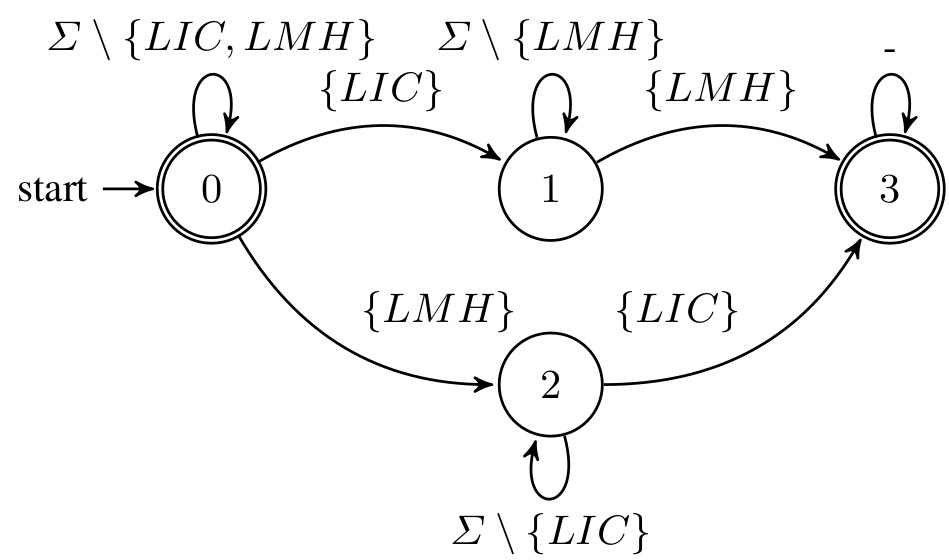
\includegraphics[width=.5\textwidth]{images/m1.png}\label{fig:m1}}\quad
	\subfloat[][$\mathsf{Precedence}(\textit{SQ},\textit{RQR})$]{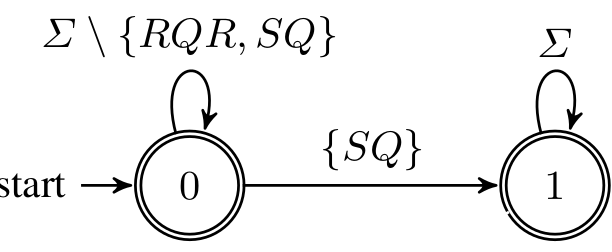
\includegraphics[width=.3\textwidth]{images/m2.png}\label{fig:m2}}\quad
	\caption{Automata generated for Declare templates using \cite{LeoniMA12,DBLP:conf/bpm/Westergaard11}}\label{fig:ma}
\end{figure}

\subsection{A$^*$ space search}
Given a Declare model $\mathcal{D}=(\Activities,\Pi)$, where $\Pi$ is a set of Declare constraints $\pi_i$ which semantics can be represented as a LTL$_f$ formula $\phi_i$ \cite{GiacomoMM14}. Each of these formulae can be represented as a single DFA$_{\phi_i}$ \cite{LeoniMA12}  using one of the algorithms proposed in \cite{DBLP:conf/bpm/Westergaard11}; these graphs are edge labelled by a set of non-negated activity labels (Figure~\ref{fig:ma}). Furthermore, a trace is valid for $\sigma\in L(\mathcal{D})$ if it is accepted by all the generated automata, i.e., $\sigma\in L(\mathcal{D})\Leftrightarrow\sigma\vDash\mathcal{D}\Leftrightarrow \forall \pi_i\in\Pi. \sigma\in L(\textup{DFA}_i) $; as a result, a model trace is the set of all the valid model traces generated by all the automata.

An alignment of a trace $\sigma$ with a declare model $\mathcal{D}$ is performed via a A* search algorithm, starting from an empty alignment $\gamma_\emptyset$. The computation halts when we reach an alignment $\gamma_{\sigma,\sigma_M}$ where $\sigma_M\in L(\mathcal{D})$. As the number of the model traces  $|L(\mathcal{D})|$  is potentially a countably infinite set, the graph for the A* is not completely constructed before running the algorithm, while it is generated while visiting the candidate neighbor nodes of the currently visited node. Given a currently visited node $\gamma_{\sigma,\varsigma}$, we could possibly move to a neighbour node $\gamma_{\sigma c,\varsigma d}$ where $(c,d)$ is a valid move. The candidate node to be visited after $\gamma_{\sigma,\varsigma}$ is elected among the nodes within a priority queue having the minimum evaluation function $f(\gamma_{\sigma,\varsigma})=g(\gamma_{\sigma,\varsigma})+h(\gamma_{\sigma,\varsigma})$, where such functions are defined as follows:
\begin{itemize}
	\item $g(\gamma_{\sigma,\varsigma})=\kappa^{\min}|\varsigma|+\mathcal{K}(\gamma_{\sigma,\varsigma})$
	\item $h(\gamma_{\sigma,\varsigma})=\underset{\sigma_M\in L (\mathcal{D}),\varsigma\subseteq\sigma_M }{\min}\kappa^{\min}(|\sigma_M|-|\varsigma|)$
\end{itemize}
In order to reduce the number of comparisons between all the automata associated to the declare model, we can potentially generate one single automaton out of the  by performing the kronecker product among all the DFA$_i$-s \cite{DBLP:conf/edbt/BergamiMM17} where we preserve the edges having no empty intersection in their labels: given two DFAs $G_1=(V_1,E_1,s_1,F_1)$ and $G_2=(V_2,E_2,s_2,F_2)$, the product DFA is $G_1\times G_2=(V_1\times V_2, E_\times,s_1\times s_2,F_1\times F_2)$, where: $E_\times = \{((a,c),(b,d))\in (V_1\times V_2)^2|(a,b)\in E_1,(c,d)\in E_2,\lambda(a,b)\cap\lambda(c,d)\neq\emptyset\}$. As a result, we do not require 
\checkmark for describing trace alignments while we can exploit string matching scoring functions \cite{CAiSE21}. The resulting graph product preserves the alignment equivalence requirements in \cite{LeoniMA12}, where further space reduction strategies are also described. 

This approach can be extended to handle Data Aware Declare models by defining $\Sigma=\Activities\cup \Activities\cdot\{\mathbf{P}_1,\dots,\mathbf{P}_n\}$, where $\{\mathbf{P}_1,\dots,\mathbf{P}_n\}$ is the set of the Data Aware Declare predicates appearing within the model of interest, and by eploiting the following cost function:
\[\kappa(a_1,a_2)=\begin{cases}
	\delta_a(a_1, \const{a}) &  a_2=\const{a}\mathbf{P} \wedge \mathbf{P}(a_1)\\
	\delta_b(a_1, \const{a}) &  a_2=\const{a}\mathbf{P} \wedge \neg\mathbf{P}(a_1)\\
	\delta_c(a_1,\const{a}) & a_2=\const{a} \\
\end{cases}\]
where $\delta_a$, $\delta_b$, and $\delta_c$ are cost functions among strings over three different scenarios. 

\begin{figure}[!t]
	\centering
	\subfloat[][$\mathsf{CoExistence}(\textit{LIC},\textit{LMH})$]{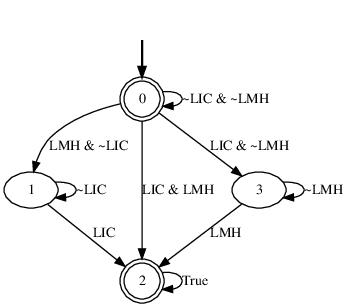
\includegraphics[width=.5\textwidth]{images/g1.png}\label{fig:vm1}}\quad
	\subfloat[][$\mathsf{Precedence}(\textit{SQ},\textit{RQR})$]{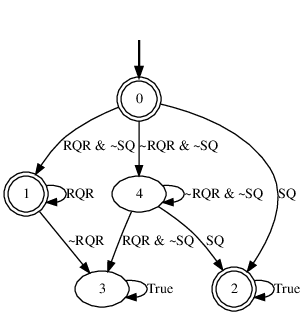
\includegraphics[width=.45\textwidth]{images/g2.png}\label{fig:vm2}}\quad
	%\subfloat[][$\square((\const{a}\wedge \mathbf{P}_1)\Leftrightarrow \lozenge(\neg\const{b}\wedge \neg\mathbf{P}_2))$]{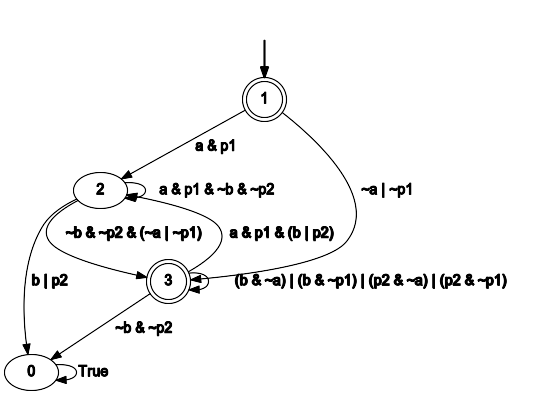
\includegraphics[width=.5\textwidth]{images/img3.png}\label{<figure3>}}
	\caption{Automata generated for Declare templates using \cite{GiacomoV13,GiacomoMM14}}\label{fig:mma1}
\end{figure}
\begin{figure}
	\centering
	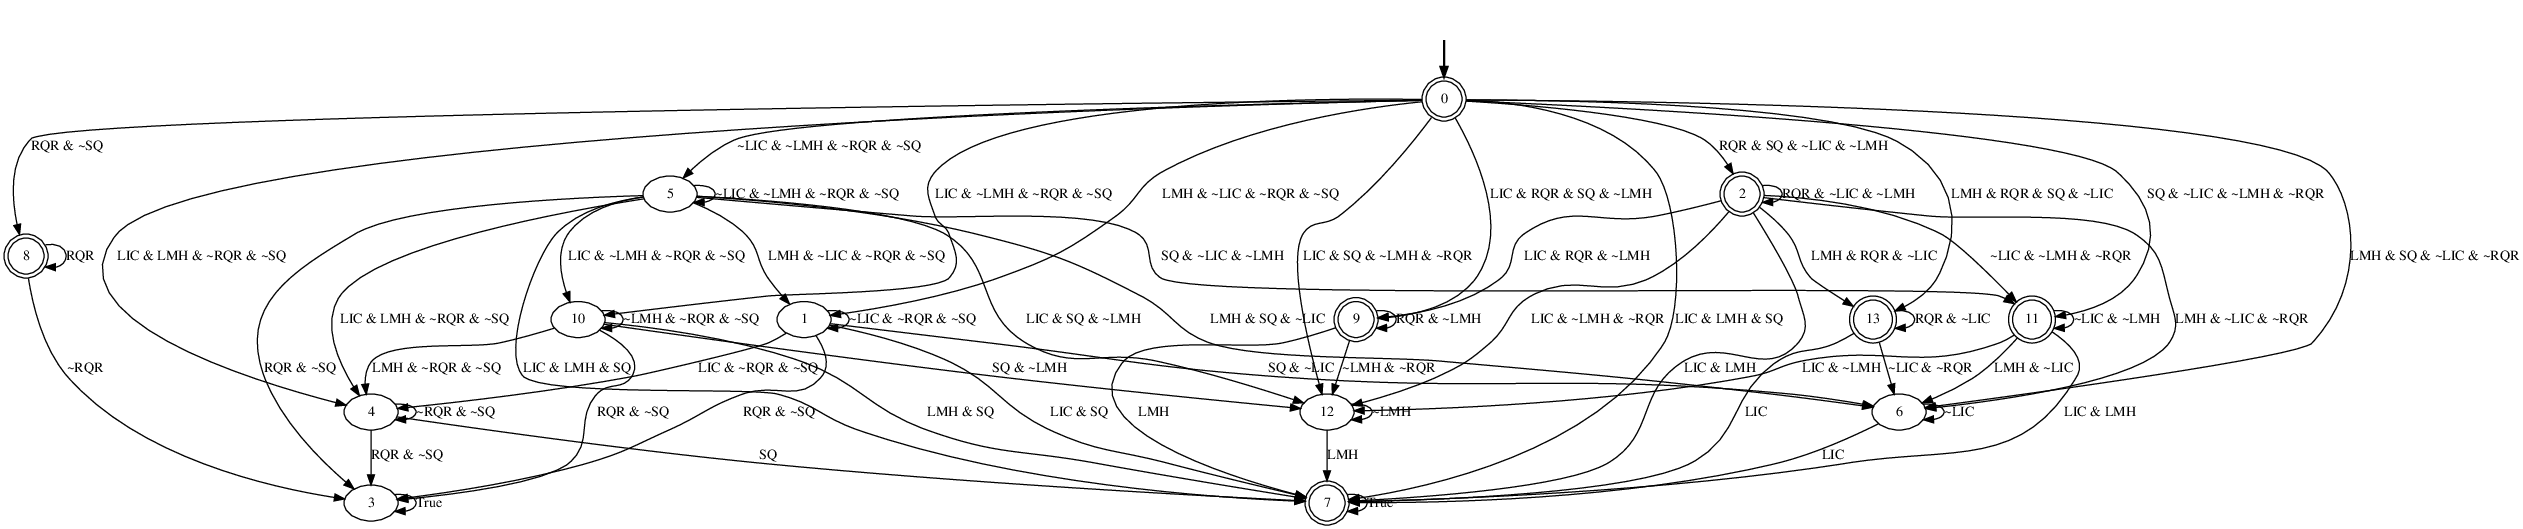
\includegraphics[width=\textheight,angle=90]{images/g3.png}\caption{Automata for $\mathsf{CoExistence}(\textit{LIC},\textit{LMH})\wedge\mathsf{Precedence}(\textit{SQ},\textit{RQR})$ generated using using \cite{GiacomoV13,GiacomoMM14}}\label{fig:mma2}\quad
\end{figure}
\subsection{Approximate Graph Matching}\label{ref:agm}
Given that the previous approach requires an heuristic for determining the best alignment of a trace, we want to identify an algorithm providing the best alignment in polynomial time, without necessarily pruning a potentially infinite search space and by exploiting no heuristic functions. 

The semantics of Declare models can be expressed as a single LTL$_f$ formula $\phi$: in particular, we can represent each of these  as a single NFA$\phi$, such that $\sigma\vDash\phi\Leftrightarrow \sigma\in L(\textup{NFA}_\phi)$ \cite{GiacomoV13,GiacomoMM14}, where $L(\textup{NFA}_\phi)$ is the language generated by $\textup{NFA}_\phi$ (Figure~\ref{fig:mma1} and \ref{fig:mma2}). Given a set of atomic tasks $\Activities$, $\textup{NFA}_\phi$ is a graph, where  the nodes represent the formulae that are valid for all the traces that are accepted starting from this node, and  edges are labelled with  a combination of predicates $\mathcal{P}=\Activities$ in disjunctive normal form: edges can be traversed only if the currently-visited event satisfies the associated condition. This problem formulation does not allow to perform trace alignments, as the testing condition is a boolean condition. 


On the other hand, it is always possible to approximately align a trace $\sigma$ to a node-labelled automaton $N$ having one single accepting (and initial) state \cite{Myers1989}. Given that it is always possible to transform a $\textup{NFA}_\phi$ to a node-labelled graph \cite{CAiSE21} as required by \cite{Myers1989}, the algorithm starts by transforming a trace $\sigma$ to a node-labelled path $P_{\tau\sigma}$; given $N$, it generates a novel automaton $P_\sigma\square N$, which initial (accepting) state is the node-pair representing the initial (accepting) states for both automata, and $\square$ is the graph cartesian product \cite{10.5555/2031398}. Next, we annotate each edge as either a deletion, an insertion, a substitution, or a null (no mis-alignment) edge with possibly arbitrary alignment costs: as a result, all the paths between the initial state and the final state of $P_\sigma\square N$ represent all the possible alignments between $\sigma$ and the sequences of $L(A_\phi)$, and the shortest path models the minimum alignment. Please observe that, by construction, a minimum-weight path may be found by considering only those paths that are cycle free \cite{10.5555/2031398}. Consequently, this problem reduction proves that the alignment of a trace against a declare model can be performed in polynomial time over the size of the data and in exponential time over the size of the query, similarly to the query semantics of SQL queries \cite{DBLP:conf/stoc/Vardi82}.

Albeit NFAs generated in \cite{GiacomoV13,GiacomoMM14} mainly refer to usual Declare models, such solution can be also extended to Data Aware Declare models by extending $\mathcal{P}$ with the data predicates $\{\mathbf{P}_1,\dots,\mathbf{P}_n\}$ within the Data Aware Delcare model of interest.

Please observe that this solution limits the expressivity of the nodes predicates to conditions $\mathbf{P}_i$ that can be only verified over one single event. In fact, the predicates associated to each edge can be only tested over the event currently accessed while visiting the automata, as NFAs have neither registers nor stacks to remember a payload coming from a previously accepted event. Consequently, join conditions among events cannot be expressed \cite{SchonigCMM16}. \texttt{\color{red}[TODO: can we possibly represent join conditions among traces' events by changing the way\\ for which the NFA is generated from LTL$_f$? Does the representation\\ of join conditions necessarily requires Büchi automata?]} For this reason, we propose a data-driven solution, where join condition can be naturally expressed.


%Domanda: il tool \url{https://flloat.herokuapp.com/} ha generato il seguente automa per 



%
%\section{Introduction}
\label{sec:introduction}

\textit{Conformance checking} is a branch of process mining  assessing whether a sequence of distinguishable events (i.e., a \textit{trace}) conforms to the expected process behavior represented as a \textit{process model} \cite{RozinatA08}. When a trace does not conform to the model, we say that the trace is \textit{deviant}. In this case, techniques based on cost-driven alignments additionally provide minimal repair strategies to make the trace conformant to the model \cite{LeoniA13}. Alignments represent a valuable instrument for business analysts, as the combined provision of alternative repair strategies to make a trace conformant ranked by alignment cost supports the business analyst in choosing among different process improvement strategies. In conformance checking, models can be described by either procedural \added{(e.g., safe Petri Nets)} or declarative languages \added{(e.g., Data-Aware Declare)} \added{having a clear data-aware semantics};  while the former fully enumerate the set of all the possible allowed traces, the latter \deleted{provide a compact process representation by} list\deleted{ing} the constraints delimiting the expected behavior \cite{LeoniA13,Westergaard11}. Nevertheless, \deleted{LTL$_f$-based} declarative models expressed in \added{Linear Time Logic on Finite Traces (LTL$_f$)} can always be transformed into procedural via their associated constraint automata. \added{As LTL$_f$ is an extension of modal logic in which worlds are organized in an finite linear structure, this logic is well suited to describe business processes logs having traces of finite length \cite{GiacomoV13}.}

%In fact, such semantics describes the actions that will follow when some pre-conditions are met \cite{LiPZVR20}.
The representation of declarative process models as automata can be adopted for aligning traces with this type of models \cite{LeoniMA12,XuLZ17a}.


Multi-perspective checking for process conformance is gaining momentum, as conformance checking techniques considering both trace types and data annotations as ``first-class citizens'' enable to discover more deviations \cite{MultiPerspective}. This reflects the essence of real-world business processes, which are inherently described by both business processes and their different domain objects \cite{PetermannJMR14} (e.g., employees, products, or orders), which can be encoded as traces and event data. While alignment-based  data-aware conformance has been already investigated in the context of procedural models, most of the conformance checking approaches for data-aware declarative models \cite{BurattinMS16,Borrego014} focus on a numerical approximation of the degree of conformance of a log trace against the model and do not provide repair strategies.

For overcoming this research gap, we propose a novel approach for aligning event logs to data-aware declarative models by reducing it to a data-agnostic alignment problem over LTL$_f$-based models. This solution exploits the following considerations: \begin{enumerate*}[label=\emph{\alph*})]
	\item \label{it1} to represent the process model, we use a sub-set of the data-aware extension of Declare presented in \cite{BurattinMS16}. After representing the data\-aware Declare model using a data\added{-}agnostic LTL$_f$ semantics,
	\item \label{it2} we exploit the data predicates in the data-aware Declare clauses to partition the data space. This provides propositions representing data in addition to event labels. Then,
	\item we combine each event label with the propositions generated in \ref{it2} and transform the model in \ref{it1} into its data-aware counterpart. The automata-based representation of such a model is used to align traces (seen as sequences of events with a payload of data attribute-value pairs) with the model. Specifically, we show that the alignment problem can \deleted{can} be expressed as a planning problem in Artificial Intelligence, which can be efficiently solved by customary planners\added{: our previous work already remarked that such algorithms outperform state-of-the-art trace alignment algorithms where data payload is not considered} \cite{XuLZ17a,LeoniM17}.
%
\added{The planner generates a} repair strategy that is able to align traces with a data-aware declarative model based on changes at the level of control flow (such as adding/deleting events) or at the level of the data flow (such as changing the attribute values attached to them).
\end{enumerate*}

The paper is structured as follows: after providing relevant related works (\S\ref{sec:related}), we introduce the notion of event log (\S\ref{ssec:elog}) and the data-aware declarative language used to represent the model (\S\ref{ssec:dad}); we also provide hints on Automated Planning, as we will later exploit the SymBA*-2 optimal planner to compute the alignments (\S\ref{ssec:ap}). These preliminary notions guide us into the definition of our  working assumptions adhering to the literature of reference (\S\ref{sec:wa}). After deep-diving into the technical details providing the solution to the data-aware declarative alignment problem (\S\ref{sec:dccap}), we benchmark SymBA*-2 over a synthetic dataset and discuss its performance in this context (\S\ref{sec:experiments}). Last, we draw our final conclusions and propose some future work (\S\ref{sec:end}).


%we draw the working assumptions jointly with the assumptions from the current literature on declarative conformance checking (\S\ref{sec:wa}). After outlining the declarative model alignment over which we want to reduce the problem (\S\ref{sec:dccap}), we deep-dive into the data-aware Declare Trace Alignment Pipeline (\S\ref{sec:dadtap}) \texttt{\color{red} [TODO: experiments? ]} Last, we draw our final conclusions and propose some future works (\S\texttt{\color{red}[TODO]}). 

%%\input{sections/02_preliminaries}
%\section{Declare Constraints Ranking}

Given that the minimum alignment cost for a Declare model $\DeclModel=(\Activities, \DeclConstr)$ over an arbitrary trace $\nonlogtrace$ can be determined by the best $\DeclModel$-trace $\logtrace\in\TraceOf{\DeclModel}$ \cite{LeoniMA12}, we can first associate to each $\logtrace\in\TraceOf{\DeclModel}$ all the Declare constraints $P\in\DeclConstr$ for which $\logtrace\vDash P$ via a function $\InvInterp{\logtrace}=\Set{P\in\DeclConstr | \logtrace\vDash P}$; then, 
we can represent all the traces $\logtrace\in\TraceOf{\DeclModel}$ and $\nonlogtrace$ as vectors  in the Euclidean Space \cite{CAiSE21}, so that the alignment can be reduced to a k-nearest neighbor search of traces inducing a ranking over a similarity function $\mathcal{R}(\logtrace,\nonlogtrace)\in[0,1]$. At this point, we can rank the constraints in $\DeclConstr$ over $\nonlogtrace$ by ensembling the normalized similarities as follows:
\[\mathcal{R}_\DeclConstr(P,\nonlogtrace)=1-\prod_{\substack{\logtrace\in\TraceOf{\DeclModel},\\ P\in\InvInterp{\logtrace}}}(1-\mathcal{R}(\logtrace,\nonlogtrace))\]

%\section{Approximate Constraint Matching}
The latter approach requires to enumerate all the possible model traces $\logtrace\in\TraceOf{\DeclModel}$: even if the constraints $P\in\Pi$ can be represented finitely, the generated traces can be both arbitrarily long and expensive to enumerate. Given that Business Process Management often handles finite process descriptions \cite{GiacomoV13} thus implying a finite interpretation of such formulae, we can represent each $P\in\Pi$ as an NFA \cite{GiacomoMM14}, which labels are logical propositions. As a next step, we can perform an approximate match of the resulting NFA with the trace $\nonlogtrace$ represented as a DAG \cite{Myers1989} by exploiting a variation of the well-known dynamic programming algorithm for string matching \cite{GALIL198833}. After extending the algorithm in \cite{Myers1989} by including the proposition evaluation as a part of the match \texttt{\color{red}[TODO]}, the outcome of such algorithm will be the $\logtrace\in\TraceOf{\DeclModel}$ providing the best match for $\nonlogtrace$ alongside its associated cost, $\mathcal{A}(\textup{NFA}_{P},\textup{DAG}_{\nonlogtrace})$. 
Please note that this approach can be exploited to rank the model constraints via $\mathcal{A}$:
\[\mathcal{R}_{\mathcal{A}}(P,\nonlogtrace)=\frac{1}{\mathcal{A}(\textup{NFA}_{P},\textup{DAG}_{\nonlogtrace})+1}\]
\subsection{Data-Driven Declare Model Mining}\label{ref:dddmm}
In some other use cases, the model $\DeclModel$ is unknown, and we want to mine the set of plausible rules from a log \cite{MaggiMA11}. In this case, we are interested in knowing which and how many log traces $\sigma_L$ satisfy (albeit approximately) a Declare constraint $P$. This requires to visit the same log dataset multiple times for multiple candidate constraints $P\in\DeclConstr$: although it already exists a previous attempt at minining declarative models via relational databases \cite{SSRSA}, state-of-the-art interpretation of relational queries face inefficient implementation of aggregation operations \cite{BergamiPM18}. It can be showed that some counting constraints (e.g., \texttt{existence}, \texttt{init}) can be efficiently computed while loading the data traces within the relational database thus avoiding the counting cost: however, the authors did not consider this possibility in their implementation. Furthermore, row-oriented systems such as the Microsoft SQL Server exploited in \cite{SSRSA} are not particularly query efficient if compared to column-based storage \cite{IdreosGNMMK12}, where each $n$-ary relation $r(\texttt{id},A_1,\dots,A_n)$ can be decomposed into $n$ relations $r_i(\texttt{id},A_i)$. Last, at the time of the writing, no relational database system is capable of running multiple queries contemporaneously while minimising the data access and visit time to the log space: in this paper, we provide a from-scratch implementation of a in-memory relational database for data-driven declare mining enabling an efficient parallel implementation of the query plan, thus making the mining of Data-Driven Declare Models particularly efficient.

$\sigma_1=\mathsf{aaab}\qquad\sigma_2=\mathsf{bbbba}\qquad\sigma_3=\mathsf{cbcbc}$
\medskip

\begin{figure}\centering
	\begin{tabular}{c|c|c}
	\toprule
	\multicolumn{3}{c}{\texttt{CountTemplate}}\\
	\toprule
	\texttt{act} & $\sigma_{\texttt{id}}$ & \texttt{count}\\
	\midrule
	$\mathsf{a}$& 1 & 3 \\
	$\mathsf{a}$& 2 & 1 \\
	$\mathsf{a}$& 3 & 0 \\
	$\mathsf{b}$& 1 & 1 \\
	$\mathsf{b}$& 2 & 4 \\
	$\mathsf{b}$& 3 & 2 \\
	$\mathsf{c}$& 1 & 0 \\
	$\mathsf{c}$& 2 & 0 \\
	$\mathsf{c}$& 3 & 3 \\
	\bottomrule
\end{tabular} \begin{tabular}{c|c|c|c|c}
\toprule
\multicolumn{5}{c}{\texttt{Act}}\\
\toprule
 \texttt{act} & $\sigma_{\texttt{id}}$ & \texttt{time} & \texttt{next} & \texttt{prev}\\
\midrule
 $\mathsf{a}$ &1 & 0.00 &  2 & $-\infty$\\ 	%1	1
 $\mathsf{a}$ &1 & 0.33 &  3 & 1\\ 			%2	2
 $\mathsf{a}$ &1 & 0.66 &  \textbf{5} & 2\\ 			%3	3
 $\mathsf{a}$ &2 & 1.00 &  $+\infty$ & \textbf{9}\\ 	%9	4
 $\mathsf{b}$ &1 & 1.00 &  $+\infty$ & 3\\	%4	5
 $\mathsf{b}$ &2 & 0.00 &  \textbf{7} & $-\infty$\\ 	%5	6
 $\mathsf{b}$ &2 & 0.25 &  \textbf{8} & \textbf{6}\\ 			%6	7
 $\mathsf{b}$ &2 & 0.50 &  \textbf{9} & \textbf{7}\\ 			%7	8
 $\mathsf{b}$ &2 & 0.75 &  \textbf{4} & \textbf{8}\\ 			%8	9
 $\mathsf{b}$ &3 & 0.25 &  \textbf{13} & \textbf{12}\\ 		%11	10
 $\mathsf{b}$ &3 & 0.75 &  14 & \textbf{13}\\ 		%13	11
 $\mathsf{c}$ &3 & 0.00 &  \textbf{10} & $-\infty$\\ %10	12
 $\mathsf{c}$ &3 & 0.50 &  \textbf{11} & \textbf{10}\\ 		%12	13
 $\mathsf{c}$ &3 & 1.00 &  $+\infty$ & \textbf{11}\\ %14	14
\bottomrule
\end{tabular} \begin{tabular}{c|c|c}
\toprule
\multicolumn{3}{c}{\texttt{AttributeK}$_i$\quad($\mathbf{P}$)}\\
\toprule
 \texttt{act} & \texttt{value} & \texttt{ActOffset}\\
 \midrule
 $\cdots$ & $\cdots$ & $\cdots$\\

\bottomrule
\end{tabular}\end{figure}

In the following expressions, the alignment returns a pair, where the first element is the candidate trace for a model, and the second argument is the alignment similarity.
\begin{itemize}

\item $\mathcal{A}(\mathsf{init}(A),\mathcal{L})=\pi_{\sigma_{\texttt{id}},\tilde{{t}}}(\textit{Calc}_{{\tilde{{t}}}:=1-\texttt{time}}(\sigma_{\texttt{act}=A}(\texttt{Act}))$
\item $\mathcal{A}(\mathsf{end}(A),\mathcal{L})=\pi_{\sigma_{\texttt{id}},\texttt{time}}(\sigma_{\texttt{act}=A}(\texttt{Act})))$
\item $\mathcal{A}(\mathsf{exactly}(A,n),\mathcal{L})=\pi_{\sigma_{\texttt{id}},\tilde{t}}(\textit{Calc}_{\tilde{t}:=1-\frac{|n-\texttt{count}|}{\mathsf{len}(\sigma_\texttt{id})}}(\sigma_{\texttt{act}=A}(\texttt{CountTemplate})))$
\item $\mathcal{A}(\mathsf{existence}(A,n),\mathcal{L})=\pi_{\sigma_{\texttt{id}},\tilde{t}}(\textit{Calc}_{\tilde{t}:=|\texttt{count}\geq n|\texttt{?}\;1\;\texttt{:}1-\frac{|n-\texttt{count}|}{\mathsf{len}(\sigma_\texttt{id})}}(\sigma_{\texttt{act}=A}(\texttt{CountTemplate})))$
\item \begin{align*}
\mathcal{A}(\mathsf{respexistence}(&A,B,\mathbf{P}),\mathcal{L})\\
&=\mathsf{notexists}^1(A)\oplus\mathsf{ifte}_{\sigma\mapsto(A\wedge \mathbf{P})(\sigma)}(\mathsf{exists}^1(B){\color{red}\oplus\mathsf{notexists}^{c}(B)},\;\top^1)
\end{align*}
\end{itemize} {\color{red}with $c\in[0,1]\subseteq\mathbb{R}_{\geq 0}$}


\begin{align*}
\mathsf{respexistence}(A,B,\mathbf{P})&=\Diamond(A\wedge \mathbf{P})\Rightarrow\Diamond B\\
	&=\sigma\mapsto [\exists t. \lambda(\sigma_t)=A\wedge \mathbf{P}(\sigma_t)]\Rightarrow [\exists t. \lambda(\sigma_t)=B]\\
	&=\sigma\mapsto\texttt{if}\;{|\Set{t\leq |\sigma|\;|\;\lambda(\sigma_t)=A}|=0}\;\texttt{then}\\
	&\qquad\qquad \texttt{return}\;1\\
	&\qquad\quad\;\; \texttt{else if}\; \lambda(\sigma_t)=A\wedge\mathbf{P}(\sigma_t)\;\texttt{then}\\
	&\qquad\qquad \texttt{return\;\{\;if}\;(\exists t.\lambda(\sigma_t)=B)\;   \texttt{then}\;1\;\texttt{else}\;{\color{red}c}\texttt{\}}\\
	&\qquad\quad\;\; \texttt{else return}\;1\\
\end{align*}
\[\mathsf{exists}^i(A)=\Set{\braket{i,l}|l\in\pi_{\sigma_{\texttt{id}}}(\sigma_{\texttt{act}=A\wedge \texttt{count}\neq0}(\texttt{CountTemplate}))}\]
\[\mathbf{P}=\bigwedge_{\texttt{K}_i\theta} \mathbf{P}_{\texttt{K}_i\theta}=\bigcap \sigma_{\mathbf{P}_{\texttt{K}_i\theta}}(\texttt{AttributeK}_i)\]
\[\mathsf{notexists}^i(A)=\Set{\braket{i,l}|l\in\pi_{\sigma_{\texttt{id}}}(\sigma_{\texttt{act}=A\wedge \texttt{count}=0}(\texttt{CountTemplate}))}\]

$\oplus$ is the disjoint union, i.e., it assumes that the left and the right operands have no elements in common, so that the weighted union of two sets $A\oplus B$ is defined as follows:
\[A\oplus B=\Set{\braket{a,p}|\braket{a,p}\in A\veebar \braket{a,p}\in B}\]
The intersection of two weighted set is the following:
\[A\cap B=\Set{\braket{a,pq}|\braket{a,p}\in A \wedge \braket{a,q}\in B}\]
Still, this definition of intersection excludes the elements satisfying either $A$ or $B$, thus only including traces satisfying both constraints. In order to overcome to this limitation, we can provide the following definition of n-ary set intersection:
\[\bigcap_n S_n = \Set{\Braket{a,\frac{1}{n}\sum_{\braket{a,p_i}\in S_i}^{i\leq n}p_i}|\exists j\leq n. \braket{a,\_}\in S_j}\]





%%\section{Declare Constraints Ranking}

Given that the minimum alignment cost for a Declare model $\DeclModel=(\Activities, \DeclConstr)$ over an arbitrary trace $\nonlogtrace$ can be determined by the best $\DeclModel$-trace $\logtrace\in\TraceOf{\DeclModel}$ \cite{LeoniMA12}, we can first associate to each $\logtrace\in\TraceOf{\DeclModel}$ all the Declare constraints $P\in\DeclConstr$ for which $\logtrace\vDash P$ via a function $\InvInterp{\logtrace}=\Set{P\in\DeclConstr | \logtrace\vDash P}$; then, 
we can represent all the traces $\logtrace\in\TraceOf{\DeclModel}$ and $\nonlogtrace$ as vectors  in the Euclidean Space \cite{CAiSE21}, so that the alignment can be reduced to a k-nearest neighbor search of traces inducing a ranking over a similarity function $\mathcal{R}(\logtrace,\nonlogtrace)\in[0,1]$. At this point, we can rank the constraints in $\DeclConstr$ over $\nonlogtrace$ by ensembling the normalized similarities as follows:
\[\mathcal{R}_\DeclConstr(P,\nonlogtrace)=1-\prod_{\substack{\logtrace\in\TraceOf{\DeclModel},\\ P\in\InvInterp{\logtrace}}}(1-\mathcal{R}(\logtrace,\nonlogtrace))\]

%%\input{sections/03_embedding_2}
%%\input{sections/05_experiment}
%%\input{sections/06_conclusion}


\bibliographystyle{splncs04}
\bibliography{biblio3}
%,bibliography2,references,libraryFiltered,main,Bibliography-CDC,DiCiccio,biblio}

\appendix 


\counterwithin{lemma}{section}
\renewcommand{\thelemma}{\thesection\arabic{lemma}}

\section{Appendix}




\end{document}
